\documentclass[9pt]{article}
\usepackage{graphicx}
\usepackage{hyperref}
\usepackage{caption}
\usepackage{amsmath}
\usepackage{mathtools}
\usepackage{physics}
\usepackage{listings}
\usepackage{xcolor}
\usepackage{subfig}
\newcommand{\numpy}{{\tt numpy}}    % tt font for numpy

\topmargin -.5in
\textheight 9in
\oddsidemargin -.25in
\evensidemargin -.25in
\textwidth 7in

\graphicspath{ {./imgs/}
               {../} }

\begin{document}

% ========== Edit your name here
\author{Due on April 8, 2022}
\title{CS 498: Assignment 4: Segmentation}
\date{March 25, 2022}
\maketitle

\medskip


\section*{Submission}
In this assignment, you will implement semantic segmentation using neural networks. The starter code consists of an iPython notebook "mp4.ipynb" which can be opened and run on Google colab. Please put together a single PDF with your answers and figures for each problem, and submit it to Gradescope (Course Code: JBXJVZ). 
We recommend you add your answers to the latex template files we provided. More details on what to report are in the provided notebook. 

Reminder: please put your name and netid in your pdf.
Your submission should include your pdf and filled out mp4.ipynb.

\section*{Semantic Segmentation} 

\paragraph{Question 1 (Data loading and augmentation)[1 pt]:}
We provide code that loads the segmentation data. In this part you will need to perform data augmentation on the loaded data within the "SegmentationDataset" class. In particular you should take a random crop of the image and with some probability you should flip the image horizontally. You should experiment with different probabilities and crop sizes and report the results in your pdf. Make sure to use pytorch built in transforms methods.
\paragraph{Answer:} 
\begin{quote}

Below is the implementation of \texttt{SegmentationDataset} class with random transform on the given image data for data augmentation.

\begin{lstlisting}[language=Python, basicstyle=\scriptsize]
if self.transform:
# -------------------------
# apply random resized crop
i, j, h, w = transforms.RandomResizedCrop.get_params(img, scale=(0.8,1), ratio=(3/4,4/3))
img = TF.resized_crop(img, i, j, h, w, (img.size[1], img.size[0]))
gt = TF.resized_crop(gt, i, j, h, w, (gt.size[1], gt.size[0]))

# apply random horizontal flip
if random.random() < 0.5:
    img = TF.hflip(img)
    gt = TF.hflip(gt)
# -------------------------
\end{lstlisting}

\texttt{transforms.RandomResizedCrop.get\_params()} generates transform parameters within the range of the given scaling factors (\texttt{scale}) and aspect ratio (\texttt{ratio}) parameters at random, where \texttt{i}, \texttt{j}, \texttt{h}, and \texttt{w} stands for the upper pixel coordinate, left pixel coordinate, height of the cropped image, and width of the cropped image, respectively. These parameters are applied to both \texttt{img} and \texttt{gt} so that both data can be transformed identically. Horizontal flipping is also applied by generating random number between 0 and 1 using \texttt{random.random()}; hence, the if statement \texttt{if random.random() < p} means the flipping is conducted with a chance of \texttt{p}. 

Fig.~\ref{fig:transform} is comparison of transformed images (a) when no transform is applied, (b) scaling is applied (\texttt{scale=(0.08, 1.0)}), (c) aspect ratio is applied (\texttt{ratio=(3/4, 4/3)}), and (d) horizontal flipping is applied (\texttt{if random.random() < 0.5}). 

I decided to use \texttt{scale=(0.8, 1.0)}, \texttt{ratio=(3/4, 4/3)}, and \texttt{random.random() < 0.5} for data augmentation by default, as those are also the default setup for data augmentation in the off-the-shelf Pytorch dataloader classes except for the scaling factor, which is \texttt{scale=(0.08, 1.0)}; this is because I hypothesize its lower bound in default (0.08) is small and hence may yield too tiny tranformed image to represent the semantic segmentation dataset for a successful training of the model that we are aiming for. 

\begin{figure}[h]
    \centering
    \subfloat [\centering default]{{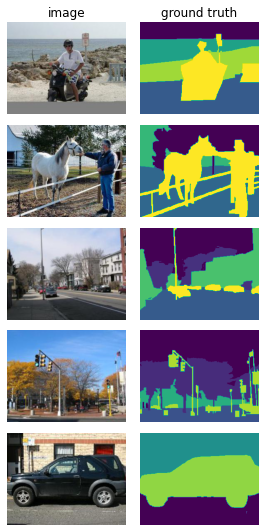
\includegraphics[width=0.24\linewidth]{default.png}}}
    % \quad
    \subfloat [\centering scaling]{{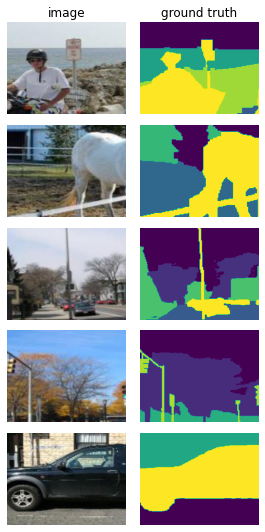
\includegraphics[width=0.24\linewidth]{scale_008_100_ratio_1_flip_0.png}}}
    % \quad
    \subfloat [\centering aspect ratio]{{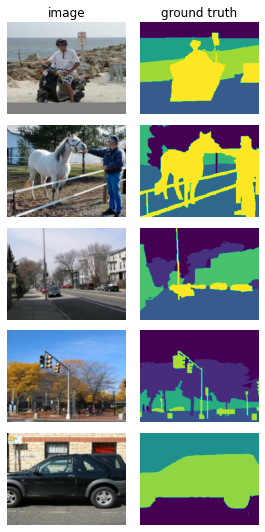
\includegraphics[width=0.24\linewidth]{scale_080_100_ratio_3_4_flip_0.png}}}
    % \quad
    \subfloat [\centering flipping]{{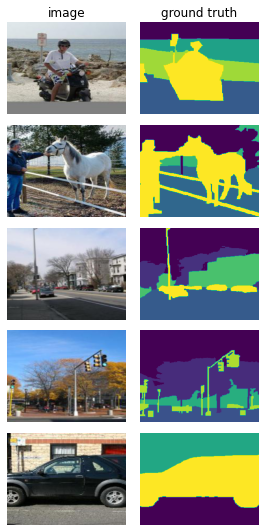
\includegraphics[width=0.24\linewidth]{scale_100_100_ratio_1_flip_50.png}}}
    \caption{Comparisons of image samples when (a) no transform, (b) scaling, (c) change in aspect ratio, and (d) horizontal flipping is applied.}
    \label{fig:transform}
\end{figure}

\end{quote}

\paragraph{Question 2 (Simple Baseline) [2 pts]:} 
In this part you will be modifying "simple\_train" and "simple\_predict". For each pixel you should compute the distribution of class labels at that pixel from the training dataset. When predicting classes for a new image, simply output these class frequencies at each pixel. You can run the evaluation code (from the next question) with your simple baseline and see its mean average precision which we provide - it should be around 24.
\paragraph{Answer:} 
\begin{quote}

Below is the implementation of \texttt{simple\_train} function, which simply counts the frequencies of classes appearing on all images at every pixel accross the training dataset.

\begin{lstlisting}[language=Python, basicstyle=\scriptsize]
# Question 2
# Output shape: (num_classes, 224, 288)
def simple_train(num_classes, train_dataloader):
    # -------------------------
    model = torch.zeros(num_classes, 224, 288)

    for i, (img, gt) in enumerate(dataloader):
        for class_label in range(num_classes):
            model[class_label] += (gt[:, 0] == class_label).sum(dim=0)

    # normalize
    model /= model[:,0,0].sum()
    model = model.numpy()
    # -------------------------
    return model
\end{lstlisting}

Below is the implementation of \texttt{simple\_predict} function, which returns the outcome of the aforementioned \texttt{model} along with ground truths given the test dataset. Note that it returns the same prediction regardless of the query images being tested.

\begin{lstlisting}[language=Python, basicstyle=\scriptsize]
# Output:
#   gt: the ground truth segmentation, shape (B, 1, 224, 288)
#   preds: the predicted segmentation class probabilities, shape (B, 9, 224, 288) 
def simple_predict(dataloader, model):
    gts, preds = [], []
    for i, batch in enumerate(dataloader):
        # -------------------------
        img_batch, gt_batch = batch
        
        for j in range(len(batch)):
            gts.append(gt_batch[j].numpy())
            preds.append(model)
        
        # -------------------------
    return np.array(gts), np.array(preds), list(dataset.classes)
\end{lstlisting}

Below table shows the reported average precision (AP) and intersection of unit (IoU) of the prediction in the aforementioned \texttt{simple\_train()} model across all nine classes, along with its visualization in Fig.~\ref{fig:simple-predict}. Note that the mean average precision (mAP) is reported as 0.24, which is in line with the given information brought up in the question. Also, the visualization results poorly distinguishes different classes such as sky, tree, or ground. Again, this is less meaningful as all queries should return the same outcome.

% prediction results
{\centering \tt \small
sky: AP: 0.60, IoU: 0.63 \\
tree: AP: 0.15, IoU: 0.00 \\
road: AP: 0.52, IoU: 0.96 \\
grass: AP: 0.12, IoU: 0.00 \\
water: AP: 0.18, IoU: 0.00 \\
building: AP: 0.42, IoU: 0.54 \\
mountain: AP: 0.01, IoU: 0.00 \\
foreground: AP: 0.18, IoU: 0.26 \\
misc: AP: 0.03, IoU: 0.00 \\
mean: AP: 0.24, IoU: 0.27 \\
}

% outcome of simple prediction
\begin{figure}[h]
    \centering
    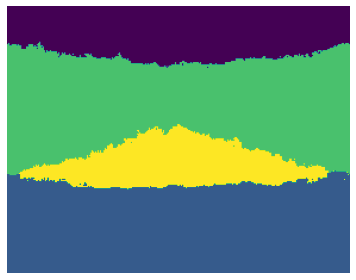
\includegraphics[width=0.5\linewidth]{simple_predict.png}
    \caption{Results of the simple prediction algorithm.}
    \label{fig:simple-predict}
\end{figure}

\end{quote}

\paragraph{Question 3 (Evaluation Metrics) [1 pts]:}  
We must evaluate the quality of our predictions. In this part you will fill in "compute\_confusion\_matrix". You should write code to compute the confusion matrix as well as IoU for the predicted segmentation when compared to ground truth. We provide code for visualizing the computed values as well as computing mean average precision.
\paragraph{Answer:} 
\begin{quote}

Below is the implementation of computing the confusion matrix and intersection of unit (IoU) as a byproduct, given the pair of prediction and ground truth of semantic segmentation. 

\begin{lstlisting}[language=Python, basicstyle=\scriptsize]
# Question 3: compute the confusion matrix and IoU metrics
# Hint: once you've computed the confusion matrix, IoU is easy
# Note: preds contains class probabilities, convert this to a class prediction
def compute_confusion_matrix(gts, preds):
    # --------------------------
    n_classes = 9
    conf = np.zeros((n_classes, n_classes))
    IoU = np.zeros((n_classes))
    
    gts_argmax = gts[:,0]
    preds_argmax = np.argmax(preds, axis=1)

    for i in range(n_classes):
        for j in range(n_classes):
            conf[i][j] = np.count_nonzero((gts_argmax==i)*(preds_argmax==j))
    
    IoU = conf.diagonal() / conf.sum(axis=1)
    # --------------------------
    return IoU, conf
\end{lstlisting}

Note that computing IoU becomes trivial after the confusion matrix is constructed. Fig.~\ref{fig:eval-simple-predict} is the visualization of the confusion matrix with for the aforementioned simple model yield by running \texttt{simple\_train()} function on the given training dataset. Note that the mAP and mIoU are the same to the reported results in Question 2.

% visualization of confusion matrix
\begin{figure}[h]
    \centering
    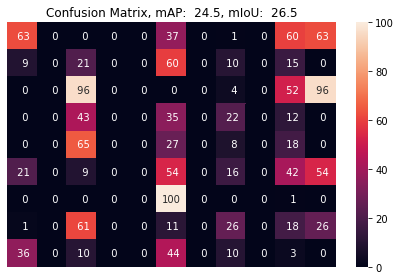
\includegraphics[width=0.5\linewidth]{eval_simple_predict.png}
    \caption{Evaluation on the results of the simple prediction.}
    \label{fig:eval-simple-predict}
\end{figure}

\end{quote}

\paragraph{Question 4 (Loss function) [2 pt]:} 
To train a model we need a loss function. In this part you will fill in "cross\_entropy\_criterion" with your implementation of the weighted cross entropy between predicted class probabilities and ground truth class labels.
\paragraph{Answer:} 
\begin{quote}

Below is the implementation of the weighted cross entropy between predicted class probabilities and ground truth class labels.

\begin{lstlisting}[language=Python, basicstyle=\scriptsize]
def cross_entropy_criterion(predictions, labels, weights, device):
    # https://pytorch.org/docs/stable/generated/torch.nn.CrossEntropyLoss.html#torch.nn.CrossEntropyLoss
    # https://gist.github.com/yang-zhang/217dcc6ae9171d7a46ce42e215c1fee0
    
    B, C, H, W = predictions.shape

    if type(predictions) is not torch.Tensor:
        predictions = torch.from_numpy(predictions)
    if type(labels) is not torch.Tensor:
        labels = torch.from_numpy(labels)

    pred = predictions.reshape(B,C,-1).to(device)
    target = labels.reshape(B,-1).to(device)

    pred = F.log_softmax(pred, dim=1)
    loss = F.nll_loss(pred, target, torch.FloatTensor(weights).to(device))

    return loss
\end{lstlisting}

The (categorical) cross entropy is a softmax activation---which has a role of encoding the arbitrary set of numbers into a normalized form so that it seems like a probability mass function---followed by the negative log-likelihood minimization---an optimization that penalizing non-similarity between two distributions. As a result, minimizing the cross entropy loss has an effect of similarizing the distribution of prediction to that of the ground-truth. Weight, which is derived by taking the inverse of class's frequencies in the dataset, has an impact of penalizing losses corresponding to the classes frequently appear, and vice versa; as a result, the classes rarely exist are considered more significantly so that the training model identifies them well.

\end{quote}

\paragraph{Question 5 (Train loop) [2 pt]:} 
In this part you will implement the stochastic gradient descent training loop in pytorch, modifying "train". We provide code to validate a trained model and a skeleton for training one. 
\paragraph{Answer:} 
\begin{quote}

Below is the implementation of the training loop for the deep-learning-based semantic segmentation model.

\begin{lstlisting}[language=Python, basicstyle=\scriptsize]
def train(model, optimizer, criterion, trainloader, device, 
            scheduler=None, epochs=100, num_early_stop=np.nan,
            valloader=None, save_path=MODEL_PATH):
    # -------------------------
    best_model_fname = "model_best.pth"
    best_model_path = os.path.join(save_path, best_model_fname)

    # create a directory to save checkpoints
    if not os.path.exists(save_path):
        os.makedirs(save_path)
        print("Create %s" % (save_path))
    # -------------------------
    ...
    for epoch in range(epochs):
        running_loss = 0.0
        for i, data in enumerate(trainloader, 0):
            # -------------------------
            img, gt = data
            img = img.to(device)
            gt = gt.to(device)
            
            optimizer.zero_grad()
            pred = model(img)
            loss = criterion(pred, gt).to(device)
            loss.backward()
            optimizer.step()
            running_loss += loss.item()
            # -------------------------
        ...

        if not valloader is None:
            val_loss = 0.0
            with torch.no_grad():
                for data in valloader:
                    # -------------------------
                    img, gt = data
                    img = img.to(device)
                    gt = gt.to(device)
                    
                    pred = model(img)
                    loss = criterion(pred, gt)
                    val_loss += loss.item()
                    # -------------------------
            ...
            # -------------------------
            # step over scheduler
            if not scheduler is None:
                scheduler.step(np.mean(val_loss))

            # check whether the performance has been improved. if not, quit training
            if val_loss == min(val_loss_over_epochs):
                torch.save(model.state_dict(), best_model_path)
                print(f"Epoch: {epoch+1}, Best model saved at {best_model_path}")
                num_no_improvement = 0
            else:
                num_no_improvement += 1
                print(f"Epoch: {epoch+1}, No improvement ({num_no_improvement} / {num_early_stop})")
                if num_no_improvement >= num_early_stop:
                    break
            # -------------------------
    ...
    # -------------------------
    plt.tight_layout()
    plt.savefig(os.path.join(save_path, "loss_curve.png"))
    # -------------------------
    return model
\end{lstlisting}

Monitoring both training and validation loss is important to avoid the trained model's overfitting to the training dataset, as the goal of training is to apply the model to the general cases (i.e., across among training, validation, and test sub-datasets), not confining to the training set. If the validation loss does no longer improve or even get worse while the training loss is decreasing, it implies that the model is being overfitted to the training set, which means that it is now losing its generality. This is the reason why the model showing the best validation loss is being saved, and scheduler works when the validation loss is not improving, not the loss evaluated over the training set. 

If the training and/or validation loss is not improving, it is easily diagnosed that the model is no longer being trained over the given training dataset. This is diagnozed that the optimization procedure has fallen into a local minimum or pitfall, and cannot escape from it due to the insufficient or large step size. To avoid such cases, one of actions usually considered to be taken is to apply scheduler to adjust the learning rate based on the number of epochs or allows dynamic learning rate reducing based on some validation measurements. By doing so, the model learns faster at the early phase in the training and learns finer at the late phase, hence minimizes the risk of falling into local mimima (which is suboptimal) and reachs the best outcome.

\end{quote}

\paragraph{Question 6 (Model definition and training) [4 pt]:} 
Implement a basic convolutional neural network, as well as the U-Net architecture for semantic segmentation. Train your models with the code you wrote for Question 5.
\paragraph{Answer:} 
\begin{quote} 

Below is the implementation of the basic convolutional neural network (CNN) blocks constructing both \texttt{BaseConv} and \texttt{UNet} segmentation model. \texttt{ConvBlock} class is a combination of a CNN layer, activation, and batch normalization. \texttt{DownConv} class is a CNN layer with downsampling, and \texttt{UpConv} is that with upsampling. \texttt{UNetUpConv}, which is a variant of \texttt{UpConv}, takes skip-connected tensor as an additional input to implement the UNet architecture.

% Basic CNN blocks
\begin{lstlisting}[language=Python, basicstyle=\scriptsize]
# credit from https://github.com/ptrblck/pytorch_misc/blob/master/unet_demo.py

# basic CNN block consisting of convnet + activation + batch normalization
class ConvBlock(nn.Module):
    def __init__(self, in_channels, out_channels, 
                    kernel_size=3, padding=1, stride=1):
        super(ConvBlock, self).__init__()
        self.conv = nn.Conv2d(in_channels, out_channels, 
                                kernel_size=kernel_size, padding=padding, 
                                stride=stride, bias=False)
        self.batch_norm = nn.BatchNorm2d(out_channels, eps=1e-05, momentum=0.1, 
                                            affine=True, track_running_stats=True)
        self.activation = nn.ReLU(inplace=True)
    
    def forward(self, x):
        x = self.conv(x)
        x = self.activation(x)
        x = self.batch_norm(x)
    
        return x

# CNN block for downsampling consisting of BaseConv followed by pooling 
# (i.e., reduce tensor side length by half)
class DownConv(nn.Module):
    def __init__(self, in_channels, out_channels, 
                    kernel_size=3, padding=1, stride=1):
        super(DownConv, self).__init__()
        self.conv_act_bn = ConvBlock(in_channels, out_channels, 
                                        kernel_size, padding, stride)
        self.pooling = nn.MaxPool2d(kernel_size=3, padding=1, stride=2, 
                                    dilation=1, ceil_mode=False)
        
    def forward(self, x):
        x = self.pooling(x)     # reduce side of tensor by half
        x = self.conv_act_bn(x)   

        return x

# CNN block for upsampling consisting of ConvTranspose2d followed by BaseConv 
# (i.e., increase tensor side length twice)
class UpConv(nn.Module):
    def __init__(self, in_channels, out_channels, 
                    kernel_size=3, padding=1, stride=1):
        super(UpConv, self).__init__()
        self.conv_act_bn = ConvBlock(in_channels, out_channels, 
                                        kernel_size, padding, stride)
        self.conv_transpose = nn.ConvTranspose2d(in_channels, in_channels, 
                                                    kernel_size=2, padding=0, 
                                                    stride=2, bias=False)
        
    def forward(self, x):
        x = self.conv_transpose(x)  # increase side of tensor twice
        x = self.conv_act_bn(x)

        return x

# CNN block for upsampling with skip connection in UNet architecture, 
# consisting of ConvTranspose2d followed by BaseConv 
# (i.e., increase tensor side length twice)
class UnetUpConv(nn.Module):
    def __init__(self, in_channels, in_channels_skip, out_channels, 
                    kernel_size=3, padding=1, stride=1):
        super(UnetUpConv, self).__init__()
        self.conv_act_bn = ConvBlock(in_channels+in_channels_skip, out_channels, 
                                        kernel_size, padding, stride)
        self.conv_transpose = nn.ConvTranspose2d(in_channels, in_channels, 
                                                    kernel_size=2, padding=0, 
                                                    stride=2, bias=False)
        
    def forward(self, x, x_skip):
        x = self.conv_transpose(x)          # increase side of tensor twice
        x = torch.cat((x, x_skip), dim=1)   # concatenate upsampled and skipped tensor
        x = self.conv_act_bn(x)             # proceed to convnet operation

        return x
\end{lstlisting}

Below is the implementation of the basic convolutional neural network with a encoder-decoder shape for semantic segmentation task. The basic model structure resembles that of ResNet-18 for a fair comparison in Question 7, except for duplicated CNN layers on each level. The tensor shape at each layer is delineated in the attached source code in jupyter notebook.

% BaseConv
\begin{lstlisting}[language=Python, basicstyle=\scriptsize]
class BaseConv(nn.Module):
def __init__(self, n_classes=9):
    super(BaseConv, self).__init__()

    in_channels = 3
    out_channels = 64

    # block for convnet operation for input tensor
    self.conv_in = ConvBlock(in_channels=in_channels, out_channels=out_channels, 
                                kernel_size=7, padding=3, stride=2)

    # blocks for convnet operation followed by downsampling
    self.conv_down1 = DownConv(in_channels=1*out_channels, out_channels=1*out_channels)
    self.conv_down2 = DownConv(in_channels=1*out_channels, out_channels=2*out_channels)
    self.conv_down3 = DownConv(in_channels=2*out_channels, out_channels=4*out_channels)
    self.conv_down4 = DownConv(in_channels=4*out_channels, out_channels=8*out_channels)

    # blocks for convnet operation preceded by upsampling
    self.conv_up4 = UpConv(in_channels=8*out_channels, out_channels=4*out_channels)
    self.conv_up3 = UpConv(in_channels=4*out_channels, out_channels=2*out_channels)
    self.conv_up2 = UpConv(in_channels=2*out_channels, out_channels=1*out_channels)
    self.conv_up1 = UpConv(in_channels=1*out_channels, out_channels=1*out_channels)
    self.conv_up0 = UpConv(in_channels=1*out_channels, out_channels=1*out_channels)
    
    # block for convnet operation to construct n_classes semantic outputs
    self.conv_out = nn.Conv2d(in_channels=out_channels, out_channels=n_classes, 
                                kernel_size=1, padding=0, stride=1)

def __repr__(self):
    return "BaseConv"
    
def forward(self, x):
    x = self.conv_in(x)
    
    x_down1 = self.conv_down1(x)
    x_down2 = self.conv_down2(x_down1)
    x_down3 = self.conv_down3(x_down2)
    x_down4 = self.conv_down4(x_down3)
    
    x_up4 = self.conv_up4(x_down4)
    x_up3 = self.conv_up3(x_down3)
    x_up2 = self.conv_up2(x_up3)
    x_up1 = self.conv_up1(x_up2)
    x_up0 = self.conv_up1(x_up1)

    pred = self.conv_out(x_up0)

    return pred
\end{lstlisting}

Below is the implementation of the UNet, an extension of the aforementioned \texttt{BaseConv} architecture with skip connection. The tensor shape at each layer is delineated in the attached source code in jupyter notebook.

% UNet
\begin{lstlisting}[language=Python, basicstyle=\scriptsize]
class UNet(nn.Module):
def __init__(self, n_classes=9):
    super(UNet, self).__init__()

    in_channels = 3
    out_channels = 64

    # block for convnet operation for input tensor
    self.conv_in = ConvBlock(in_channels=in_channels, out_channels=out_channels, 
                                kernel_size=7, padding=3, stride=2)

    # blocks for convnet operation followed by downsampling
    self.conv_down1 = DownConv(in_channels=1*out_channels, out_channels=1*out_channels)
    self.conv_down2 = DownConv(in_channels=1*out_channels, out_channels=2*out_channels)
    self.conv_down3 = DownConv(in_channels=2*out_channels, out_channels=4*out_channels)
    self.conv_down4 = DownConv(in_channels=4*out_channels, out_channels=8*out_channels)

    # blocks for convnet operation preceded by upsampling
    self.conv_up4 = UnetUpConv(in_channels=8*out_channels, in_channels_skip=4*out_channels, 
                                out_channels=4*out_channels)
    self.conv_up3 = UnetUpConv(in_channels=4*out_channels, in_channels_skip=2*out_channels, 
                                out_channels=2*out_channels)
    self.conv_up2 = UnetUpConv(in_channels=2*out_channels, in_channels_skip=1*out_channels, 
                                out_channels=1*out_channels)
    self.conv_up1 = UnetUpConv(in_channels=1*out_channels, in_channels_skip=1*out_channels, 
                                out_channels=1*out_channels)
    self.conv_up0 = UpConv(in_channels=1*out_channels, out_channels=1*out_channels)
    
    # block for convnet operation to construct n_classes semantic outputs
    self.conv_out = nn.Conv2d(in_channels=out_channels, out_channels=n_classes, 
                                kernel_size=1, padding=0, stride=1)

def __repr__(self):
    return "UNet"        

def forward(self, x):
    x = self.conv_in(x)
    x_down1 = self.conv_down1(x)
    x_down2 = self.conv_down2(x_down1)
    x_down3 = self.conv_down3(x_down2)
    x_down4 = self.conv_down4(x_down3)

    x_up4 = self.conv_up4(x_down4, x_down3)
    x_up3 = self.conv_up3(x_up4, x_down2)
    x_up2 = self.conv_up2(x_up3, x_down1)
    x_up1 = self.conv_up1(x_up2, x)
    x_up0 = self.conv_up0(x_up1)

    pred = self.conv_out(x_up0)

    return pred
\end{lstlisting}

% TODO: DESCRIBE BOTH MODELS IN DETAIL.

Below is the example code for creating, traing, and evaluating a model with a \texttt{BaseConv} instance. The model type can differ at user's convenience (e.g., one can generate a \texttt{UNet} instance instead of \texttt{BaseConv}). I clarify that the identical training setup is used thoroughout the reported results in Question 6 and 7 for a fair comparison: SGD with learning rate 1e-3 as an optimizer, 50 epochs, turning off optimizer scheduler and early stopping. It is observed that these configurations give a reasonable training results (i.e., mAP $\geq$ 0.5) across all deep-learning models we are investigating. 

% training code
\begin{lstlisting}[language=Python, basicstyle=\scriptsize]
# First make the model and put it on the device
base_model = BaseConv().to(device)

# Now define our loss criterion as cross entropy based on your previous code
criterion = lambda y_pred, y_true: cross_entropy_criterion(y_pred, y_true, class_weights, device)

# Now make our optimizer for this model
optimizer = optim.SGD(base_model.parameters(), lr=1e-3, momentum=0.9, weight_decay=0.01)

# Now train and validate
base_model = train(base_model, optimizer, criterion, dataloader, device, 
                   valloader=val_dataloader, save_path=os.path.join(MODEL_PATH, str(base_model)),
                   epochs=50, scheduler=None, num_early_stop=np.nan)
preds, gts = validate_model(val_dataloader, base_model, list(dataset.classes), device)
\end{lstlisting}

Fig.~\ref{fig:loss-BaseConv-UNet} shows the loss curve over 50 epochs while training \texttt{BaseConv} (left) and \texttt{UNet} (right) models respectively, with the aforementioned training hyperparameter setup. 

% logs of training & validation losses
\begin{figure}[h]
    \centering
    \subfloat {{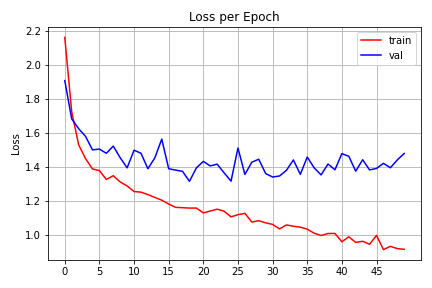
\includegraphics[width=0.45\linewidth]{loss-BaseConv.png}}}
    \qquad
    \subfloat {{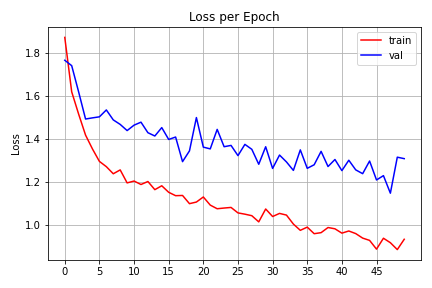
\includegraphics[width=0.45\linewidth]{loss-UNet.png}}}
    \caption{Loss curve of training \texttt{BaseConv} (left) and \texttt{UNet} (right) models, respectively.}
    \label{fig:loss-BaseConv-UNet}
\end{figure}

Below shows evaluation results of the trained \texttt{BaseConv} and \texttt{UNet} model. Both models demonstrate mAP and IoU across nine classes above 0.50, which is our minimum requirement to be achieved. Also, it is shown that \texttt{UNet} model obtains performance gain by about 0.05 in mAP and IoU compared to the \texttt{BaseConv} model, which implies that its skip connection structure helps. Also, in Fig.~\ref{fig:pred-BaseConv-UNet}, we visualize the prediction results for five different sample images in the test dataset.

% prediction results
{\centering \tt \small
\# BaseConv \\
sky: AP: 0.95, IoU: 0.90 \\
tree: AP: 0.62, IoU: 0.65 \\
road: AP: 0.90, IoU: 0.78 \\
grass: AP: 0.59, IoU: 0.71 \\
water: AP: 0.18, IoU: 0.45 \\
building: AP: 0.68, IoU: 0.55 \\
mountain: AP: 0.04, IoU: 0.28 \\
foreground: AP: 0.59, IoU: 0.56 \\
misc: AP: 0.01, IoU: 0.06 \\
mean: AP: 0.50, IoU: 0.55 \\

\# UNet \\
sky: AP: 0.95, IoU: 0.87 \\
tree: AP: 0.74, IoU: 0.75 \\
road: AP: 0.93, IoU: 0.81 \\
grass: AP: 0.72, IoU: 0.77 \\
water: AP: 0.29, IoU: 0.57 \\
building: AP: 0.74, IoU: 0.65 \\
mountain: AP: 0.06, IoU: 0.27 \\
foreground: AP: 0.68, IoU: 0.65 \\
misc: AP: 0.01, IoU: 0.09 \\
mean: AP: 0.57, IoU: 0.60 \\
}

\begin{figure}[h]
    \centering
    \subfloat {{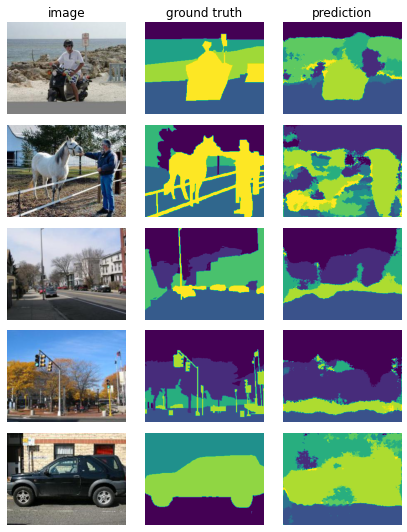
\includegraphics[width=0.45\linewidth]{pred-BaseConv.png}}}
    \qquad
    \subfloat {{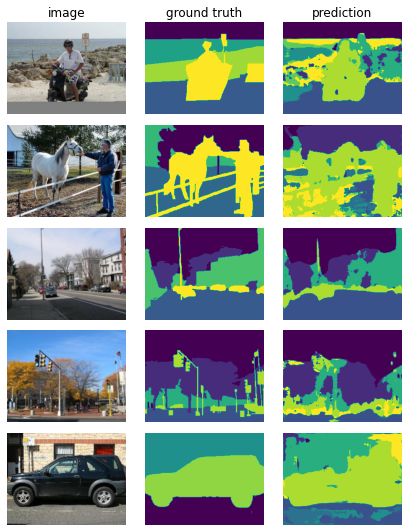
\includegraphics[width=0.45\linewidth]{pred-UNet.png}}}
    \caption{Predictions made by \texttt{BaseConv} (left) and \texttt{UNet} (right) models, respectively.}
    \label{fig:pred-BaseConv-UNet}
\end{figure}

In addition to comparing \texttt{BaseConv} and \texttt{UNet} models, I also conducted an ablation study on testing the impact of batch normalization. The tested case was a \texttt{BaseConv} model without batch normalization under the same hyperparameters and training environment. Speaking of the training speed, \texttt{BaseConv} without batch normalization slightly outperformed the vanilla \texttt{BaseConv} as both took 1135 seconds and 1217 seconds over 50 training epochs, respectively. However, as shown in the measured mAP/IoU below and visualization results along with training curve in Fig.~\ref{fig:ablation-study}, the model was hardly trained anything. From this, we realize that batch normalization plays an crucial role while training a CNN-based model.

% prediction results
{\centering \tt \small
sky: AP: 0.16, IoU: 0.00 \\
tree: AP: 0.18, IoU: 0.00 \\
road: AP: 0.21, IoU: 0.00 \\
grass: AP: 0.15, IoU: 0.00 \\
water: AP: 0.08, IoU: 0.00 \\
building: AP: 0.25, IoU: 1.00 \\
mountain: AP: 0.03, IoU: 0.00 \\
foreground: AP: 0.15, IoU: 0.00 \\
misc: AP: 0.01, IoU: 0.00 \\
mean: AP: 0.14, IoU: 0.11 \\
}

\begin{figure}[h]
    \centering
    \subfloat {{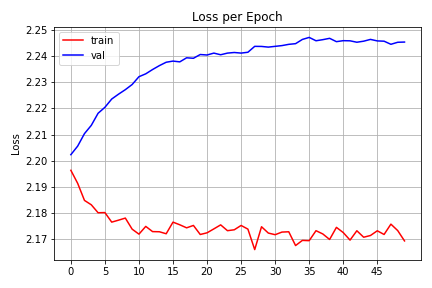
\includegraphics[height=6cm]{loss-BaseConv-no-batchnorm.png}}}
    \qquad
    \subfloat {{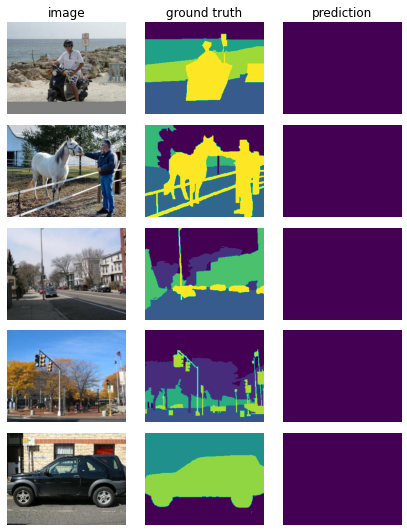
\includegraphics[height=6cm]{pred-BaseConv-no-batchnorm.png}}}
    \caption{Training curve (left) and prediction results (right) for \texttt{BaseConv} without batch normalization.}
    \label{fig:ablation-study}
\end{figure}



\end{quote}


\paragraph{Question 7 (Use Pretrained Model) [3 pt]:} 
In this part you will build on resnet-18 (note there are multiple ways to do this). Report your results, they should be better than the best you got using UNet training from scratch.
\paragraph{Answer:} 
\begin{quote}

Below is the implementation of the leveraging the pretrained ResNet-18 for a semantic segmentation task. All of its pretrained CNN layers up to having 512 channels (i.e., all layers except for pooling, linear, and activation at the end) are exploited to construct encoder shape. Both the models without having skip-connections (\texttt{ResnetBasedModel}, the counterpart of \texttt{BaseConv}) and with having skip-connections (\texttt{ResnetUNetModel}, the counterpart of \texttt{UNet}) are implemented and trained. The tensor shape at each layer is delineated in the attached source code in jupyter notebook.

Both models are trained with the same hyperparameters and setups as the \texttt{BaseConv} and \texttt{UNet} instance did: SGD with learning rate 1e-3 as an optimizer, 50 epochs, turning off optimizer scheduler and early stopping. 

% resnet-based without skip connection
\begin{lstlisting}[language=Python, basicstyle=\scriptsize]
class ResnetBasedModel(nn.Module):
def __init__(self, pretrained_resnet, num_layers_to_remove=0, n_classes=9):
    super(ResnetBasedModel, self).__init__()
    # You can, for example, extract the first N layers of the model like this:
    # self.resnet_features = nn.Sequential(*list(pretrained_resnet.children())[:N])
    
    out_channels = 64

    resnet_layers = list(pretrained_resnet.children())

    # blocks for convnet operation followed by downsampling
    self.conv_in = nn.Sequential(*resnet_layers[:3])              
    self.conv_down1 = nn.Sequential(*resnet_layers[3:5])          
    self.conv_down2 = resnet_layers[5]                            
    self.conv_down3 = resnet_layers[6]                            
    self.conv_down4 = resnet_layers[7]                            

    # blocks for convnet operation preceded by upsampling, without skip connection
    self.conv_up4 = UpConv(in_channels=8*out_channels, out_channels=4*out_channels)
    self.conv_up3 = UpConv(in_channels=4*out_channels, out_channels=2*out_channels)
    self.conv_up2 = UpConv(in_channels=2*out_channels, out_channels=1*out_channels)
    self.conv_up1 = UpConv(in_channels=1*out_channels, out_channels=1*out_channels)
    self.conv_up0 = UpConv(in_channels=1*out_channels, out_channels=1*out_channels)

    # block for convnet operation to construct n_classes semantic outputs
    self.conv_out = nn.Conv2d(in_channels=out_channels, out_channels=n_classes, 
                              kernel_size=1, padding=0, stride=1)

def __repr__(self):
    return "ResnetBasedModel"        

def forward(self, x):
    x = self.conv_in(x)
    x_down1 = self.conv_down1(x)
    x_down2 = self.conv_down2(x_down1)
    x_down3 = self.conv_down3(x_down2)
    x_down4 = self.conv_down4(x_down3)

    x_up4 = self.conv_up4(x_down4)
    x_up3 = self.conv_up3(x_up4)
    x_up2 = self.conv_up2(x_up3)
    x_up1 = self.conv_up1(x_up2)
    x_up0 = self.conv_up0(x_up1)

    pred = self.conv_out(x_up0)

    return pred
\end{lstlisting}

% resnet-based with skip connection
\begin{lstlisting}[language=Python, basicstyle=\scriptsize]
    class ResnetUNetModel(nn.Module):
    def __init__(self, pretrained_resnet, num_layers_to_remove=0, n_classes=9):
        super(ResnetUNetModel, self).__init__()
        # You can, for example, extract the first N layers of the model like this:
        # self.resnet_features = nn.Sequential(*list(pretrained_resnet.children())[:N])
        
        out_channels = 64

        resnet_layers = list(pretrained_resnet.children())

        # blocks for convnet operation followed by downsampling
        self.conv_in = nn.Sequential(*resnet_layers[:3])              
        self.conv_down1 = nn.Sequential(*resnet_layers[3:5])          
        self.conv_down2 = resnet_layers[5]                            
        self.conv_down3 = resnet_layers[6]                            
        self.conv_down4 = resnet_layers[7]                            

        # blocks for convnet operation preceded by upsampling, with skip connection
        self.conv_up4 = UnetUpConv(in_channels=8*out_channels, in_channels_skip=4*out_channels, 
                                   out_channels=4*out_channels)     
        self.conv_up3 = UnetUpConv(in_channels=4*out_channels, in_channels_skip=2*out_channels, 
                                   out_channels=2*out_channels)     
        self.conv_up2 = UnetUpConv(in_channels=2*out_channels, in_channels_skip=1*out_channels, 
                                   out_channels=1*out_channels)     
        self.conv_up1 = UnetUpConv(in_channels=1*out_channels, in_channels_skip=1*out_channels, 
                                   out_channels=1*out_channels)
        self.conv_up0 = UpConv(in_channels=1*out_channels, out_channels=1*out_channels)       

        # block for convnet operation to construct n_classes semantic outputs
        self.conv_out = nn.Conv2d(in_channels=out_channels, out_channels=n_classes, 
                                  kernel_size=1, padding=0, stride=1)
    
    def __repr__(self):
        return "ResnetUNetModel"        

    def forward(self, x):
        x = self.conv_in(x)
        x_down1 = self.conv_down1(x)
        x_down2 = self.conv_down2(x_down1)
        x_down3 = self.conv_down3(x_down2)
        x_down4 = self.conv_down4(x_down3)

        x_up4 = self.conv_up4(x_down4, x_down3)
        x_up3 = self.conv_up3(x_up4, x_down2)
        x_up2 = self.conv_up2(x_up3, x_down1)
        x_up1 = self.conv_up1(x_up2, x)
        x_up0 = self.conv_up0(x_up1)

        pred = self.conv_out(x_up0)

        return pred
\end{lstlisting}


Fig.~\ref{fig:loss-ResnetBasedModel} shows the loss curve over 50 epochs while training \texttt{ResnetBasedModel} (left) and \texttt{ResnetUNetModel} (right) respectively, with the aforementioned training hyperparameter setup. 

\begin{figure}[h]
    \centering
    \subfloat {{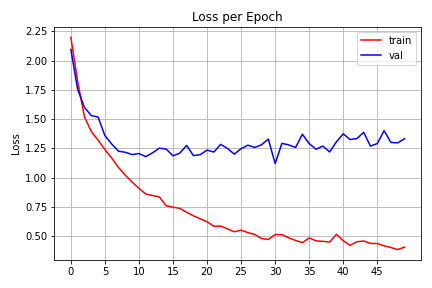
\includegraphics[width=0.45\linewidth]{loss-ResnetBasedModel.png}}}
    \qquad
    \subfloat {{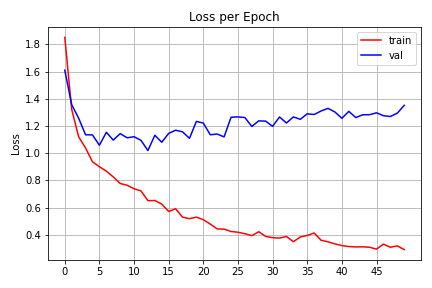
\includegraphics[width=0.45\linewidth]{loss-ResnetUNetModel.png}}}
    \caption{Loss curve of training ResNet-based models without skip connection (left) and with skip connection (right), respectively.}
    \label{fig:loss-ResnetBasedModel}
\end{figure}

Below shows evaluation results of the trained \texttt{ResnetBasedModel} and \texttt{ResnetUNetModel}. Both models demonstrate mAP and IoU across nine classes above 0.60, which have yielded performance gain by about 0.1 from their counterparts in Question 6. Also, it is shown that \texttt{ResnetUNetModel} obtains performance gain by about 0.05 in mAP and IoU compared to the \texttt{ResnetBasedModel}, which implies that the skip connection structure still helps for the model based on the pretained ResNet-18 as well. Also, in Fig.~\ref{fig:pred-ResnetBasedModel}, we visualize the prediction results for five different sample images in the test dataset.

{\centering \tt \small
\# ResnetBasedModel \\
sky: AP: 0.94, IoU: 0.84 \\
tree: AP: 0.75, IoU: 0.80 \\
road: AP: 0.94, IoU: 0.88 \\
grass: AP: 0.36, IoU: 0.50 \\
water: AP: 0.76, IoU: 0.80 \\
building: AP: 0.87, IoU: 0.76 \\
mountain: AP: 0.16, IoU: 0.31 \\
foreground: AP: 0.78, IoU: 0.70 \\
misc: AP: 0.04, IoU: 0.42 \\
mean: AP: 0.62, IoU: 0.67 \\

\# ResnetUNetModel \\
sky: AP: 0.97, IoU: 0.91 \\
tree: AP: 0.81, IoU: 0.77 \\
road: AP: 0.95, IoU: 0.86 \\
grass: AP: 0.59, IoU: 0.65 \\
water: AP: 0.67, IoU: 0.78 \\
building: AP: 0.88, IoU: 0.80 \\
mountain: AP: 0.10, IoU: 0.60 \\
foreground: AP: 0.84, IoU: 0.81 \\
misc: AP: 0.00, IoU: 0.09 \\
mean: AP: 0.65, IoU: 0.70 \\
}

\begin{figure}[h]
    \centering
    \subfloat {{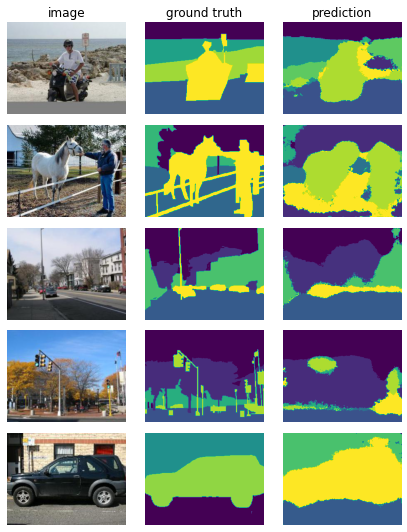
\includegraphics[width=0.45\linewidth]{pred-ResnetBasedModel.png}}}
    \qquad
    \subfloat {{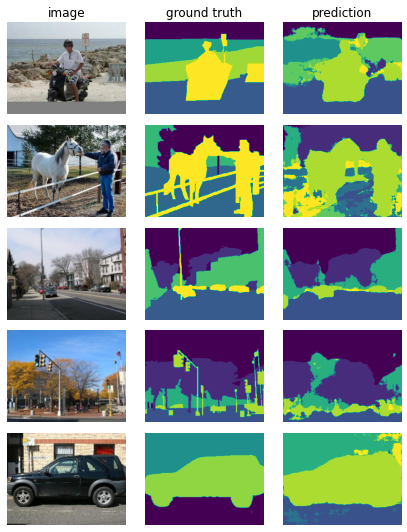
\includegraphics[width=0.45\linewidth]{pred-ResnetUNetModel.png}}}
    \caption{Predictions made by ResNet-based models without skip connection (left) and with skip connection (right), respectively.}
    \label{fig:pred-ResnetBasedModel}
\end{figure}

\end{quote}

\pagebreak

\section*{Instance Segmentation (Bonus 4pt)}

Now we have a deep semantic segmentation algorithm. However, the model cannot distinguish each instance. Could you use a similar UNet model to build an instance segmentation algorithm? Please download the Upenn-Fudan pedestrian dataset here \url{https://www.cis.upenn.edu/~jshi/ped_html/} and get their instance labels. There are two types of instance segmentation methods, detection-free or detection-based. Choose either one of them. 

Please refer to the Deep Watershed Transform for an example of detection-free method \url{https://github.com/min2209/dwt}. Your goal is to build a network with two headers, one to predict the binary semantic label similar to your semantic segmentation network and the other to predict the distance transform to the boundary. Once you have these two, the watershed transform could be applied to recover per-pixel instance labels.  

For the detection-based method, please refer to the MaskRCNN (\url{https://pytorch.org/vision/stable/_modules/torchvision/models/detection/mask_rcnn.html}). You will develop a network that predicts detection proposals first. Then within each detection proposal, a binary foreground and background segmentation is conducted to separate each instance. 

For each method, you should implement 1) the loss function the paper uses; 2) implement the data loader and post-processing that converts network output to per-pixel instance label 3) train and evaluation each model (you could either reuse your UNet backbone or follow the original paper). 

\end{document}. 

\grid
\grid